\documentclass{report}
\usepackage[english]{babel}
\usepackage{microtype}
\usepackage{amsmath,amssymb}
\usepackage{amsthm}
\usepackage[round, authoryear]{natbib}
\usepackage[all]{xy}
\usepackage{graphicx}
\usepackage{framed}
\usepackage{enumerate}
\usepackage{qtree}
\usepackage{mdframed}
\usepackage{tikz-dependency}
\usepackage{float}
\usepackage[OT2,T1]{fontenc}
\newcommand\textcyr[1]{{\fontencoding{OT2}\fontfamily{wncyr}\selectfont #1}}
\bibliographystyle{plainnat}
\author{}
\title{}

%Define theorem style for definition and metric
\theoremstyle{definition}
\newtheorem{metric}{Metric}
\newtheorem{notion}{Notion}
\theoremstyle{plain}
\newtheorem{definition}{Definition}
\def\citepos#1{\citeauthor{#1}'s (\citeyear{#1})}

%Define new float environment for tables that is boxed
\floatstyle{boxed}
\newfloat{tab}{tbp}{lop}
\floatname{tab}{Table}


\begin{document}


\chapter{Background}

Introduction to background.

\section{Machine Translation}

Machine Translation arose as a research field almost immediately after the emergence of the first computers. In these early days, several different approaches were explored. One branch of research approached translation as encoding, such models with a direct approach to translation are now known as the first generation models. Sentences were translated more or less word for word using some contextual information. Figure \ref{fig:georgetown} shows the translation of the words `much' and `many' into Russian, according to on of the early systems \citep{dostert1955georgetown}.

\begin{figure}
\begin{framed}
\footnotesize{
\begin{enumerate}
\item[1] Is the preceding word \textit{how}? (yes $\rightarrow$ \textcyr{skol\char126 ko}, no $\rightarrow$ 2)
%\item[2] \textcyr{skol\char126 ko}
\item[2] Is the preceding word \textit{as}? (yes $\rightarrow$ \textcyr{stol\char126 ko qe}, no $\rightarrow$ 3)
\item[3] Is current word \textit{much}? (yes $\rightarrow$ 5, no $\rightarrow$ 6)
\item[4] Not to be translated
\item[5] Is preceding word \textit{very} (yes $\rightarrow$ 4, no $\rightarrow$ \textcyr{mnogo})
\item[6] Is preceding word a preposition, and following word a noun? (yes $\rightarrow$ \textcyr{mnogii}, no $\rightarrow$ \textcyr{mnogo})
\end{enumerate}
}
\end{framed}
\caption{Translation of much and many from English to Russian in a direct translation system. Source: \cite[p.56]{hutchins1992introduction}.}\label{fig:georgetown}
\end{figure}

Another branch of research took a more theoretical approach involving fundamental linguistic research. The most ambitious were approaches aiming at finding an abstract meaning representation (interlingua) from the source text, and generating a target translation from this text. The results of such models were disappointing, and the general consensus in the MT community was that the less ambitious transfer approach, in which different structural representations for source and target language were used, had the best prospects for significant improvements (anders). In such transfer models, an extra stage is added to the process: the source text is first analysed into a structural representation containing information about the meaning and structure of the text and then this representation is mapped to a target side representation from which a target text can be generated. An example of a transfer rule used in the system Ariane (ref), is depicted in Figure \ref{fig:transferex}.

%better placement of arrow
\begin{figure}
\begin{framed}
\begin{tabular}{lcr}
\Tree [.\textit{supply} [.ARG0\\subj A ] [.ARG1\\obj B ] [.ARG2\\prep-obj \textit{with} C ] ] & $\rightarrow$ & \Tree [.\textit{fournir} [.ARG0\\subj A ] [.ARG2\\i-obj B ] [.ARG3\\d-obj C ] ]\\
\end{tabular}
\end{framed}
\caption{Transfer rule that accounts for the translation of `A supplies B with C' into `A fournit C a B' (accenten)}\label{fig:transferex}
\end{figure}

Although such systems were sometimes successful in small subdomains of language (e.g., \cite{chandioux1976meteo} for meteorolocial forecasts), it is very hard to formalize all of language in one system. Driven by this thought, a new line of research came of the ground, that was not primarily based on linguistic knowledge, but on large pairs of texts that were translations of each other.\footnote{Such `parallel corpora' were not created for these purposes, but existed by the grace of multilingual governments whose proceedings (?) were kept in two languages. Techniques to align these proceedings at the sentence level ... valuable data for MT research..} Corpus based models can be roughly divided into exemplar based models and statistical models. 

Exemplar based machine translation (EBMT) is directly based on analogy: sentences are translated by finding examples in the corpus similar to (fragments of) the sentence, and generate a translation by recombining them. The early EMBT researchers had the misfortune that computational standards were not as they are today, their models often treat only small sublanguages, are computationally not executable and certainly not scalable. 

The first working statistical models \citep{brown1988statistical,brown1990statistical,brown1993mathematics}, however, were ground-breaking. Although they were intrinsically word-based, the quality of their translations was an enormous improvement over any earlier model, not to mention the fact that the models, now known as `IBM model 1-5', were able to output a translation for any given input sentence (even ungrammatical ones). The statistical framework takes the view that every sentence $t$ is a possible translation of every sentence $s$. Modelling translation thus consists of modelling the probability $P(t|s)$ that $t$ is a translation of $s$, and finding the sentence $t$ for which this probability is highest. This probability distribution $P(t|s)$ has to be learned from the parallel corpus. A more detailed description of the models, as well as information on how they deal with phenomena as reordering, can be found in Section \ref{sec:IBM}.

The statistical IBM models still had the same drawbacks as the first generation of direct translation models: no structure or local context was considered, and a large amount of natural language phenomena could therefore not be accounted for. With the introduction of phrases as basic units in translation models \citep{wang1998grammar,och1999improved} a major leap forward was taken towards a proper treatment of these problem. A phrase translation pair is a pair of contiguous source and target sequences such that the words in the source phrase are aligned only with words in the target phrase, and vice versa \citep{och2000improved}. Phrases are thus not restricted to linguistic phrases, but can be any arbitrary contiguous sequence of words that is translated into a contiguous target sequence (anders). Keeping the architecture (more or less) the same, using phrases instead of words as translation units allows the model to use local context during translation. Phrase-based translation models can therefore capture short contiguous idiomatic translations, as well as small insertions and deletions and local reordering. E.g., both `a casa' and `o casa' are reasonable word for word translations of the English phrase `the house'. However, `o casa' is not a grammatical string in Portugese. The latter observation could be easily captured by a phrase-based model, as `the house' could be translated as one unit, but would be much harder to model in a word-based model. Furthermore, a word-based model would never be able to get the correct idiomatic translation of `kick the bucket' (find other example!), while a phrase-based model would have little trouble finding this translation, provided this specific idiomatic phrase was present in the training corpus. Phrase based models are discussed in more detail in Section \ref{sec:pbmodels}.

Phrase based models, although still considered state of the art, still suffer from the fact that no structure beyond the phrase level is taken into account. Approaches that addressed this problem by incorporating syntactic information to, e.g., sophisticate phrase selection of a standard phrase-based system \citep{koehn2003statistical} or rerank its output \citep{och2004alignment} were not very successful, which lead a large part of the MT community to move back to models similar to the earlier transfer based models that ruled the field before the emergence of statistical models. A major difference with the older transfer models, however, is that the newer models stayed true to the statistical and corpus based tradition, in which translation was formulated as learning a probability distribution from a parallel corpus. While the rules in the old transfer models were constructed manually, the new batch of transfer models (?) were based on the patterns found in translation corpora, making the models more scalable and robust.

There were several approaches as to detecting the patterns in translation data (anders). Some approaches first parsed the source and target text into a linguistically motivated structure and attempted to establish correspondences between the two of them (anders). This so called `parse-match-parse' method was used by, i.a., \cite{poutsma2000data}, \cite{galley2004s}, \cite{galley2006scalable} and \cite{melamed2004generalized,melamed2004statistical}, example?. As the parse-match-parse method requires fully automated parsers for both the source and target language, the number of languages pairs that can be treated as such is very limited. Furthermore, monolingual grammars are not designed for translation purposes, which makes it often very hard to find correspondences for all nodes in the tree.

A second approach is to forget about linguistic information, and concentrate on the structures suggested by the translation data. Models using this strategy are based solely on alignments (see section \ref{sec:alignments}), which describe which source words are translated into which target words, and the structures they induce (see Section \ref{sec:alignmenttrees}. As alignments generally give rise to a huge number of rules for every sentence, models using this method are hindered by computational issues. Several different solutions to restricting the rule space have been presented, in some of which formal criteria were used, while in others linguistic information was incorporated. We will discuss these methods in Section \ref{sec:SCFGs}, in which the more practical sides of such models is elaborated upon (?).

Current state of the art models ....

\newpage

\section{IBM models}
\label{sec:IBM}



\section{Phrase-based models}
\label{sec:pbmodels}

\section{Synchronous Context Free Grammars}
\label{sec:SCFGs}
 
 
\newpage
 
\section{Alignments}
\label{sec:alignments}

A word-alignment of a sentence pair is a mapping from source to target words that describes which target words are the translation of which source words (anders). Alignments can be visualized in many ways, in this thesis, we will visualize alignments using lines or arrows (see Figure \ref{fig:alignment}), in which an arrow from source word $w_s$ to target word $w_t$ thus implies that $w_t$ was involved in the translation of $w_s$.


\begin{figure}[!ht]
\centering
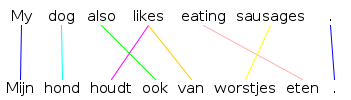
\includegraphics[scale=0.6]{alignment.png}
\caption{A one-to-many alignment of the English sentence `My dog also likes eating sausages.' and its translation `Mijn hond houdt ook van worstjes eten'.%schrijf welke tool is gebruikt
\cite{maillette2010visualizing}
%vind leuker voorbeeld: Na regen komt zonneschein, auf regen folgt sonneschein
}\label{fig:alignment}
\end{figure}


\subsection{Formally}

The precise definition of a word-alignment varies from paper to paper. Throughout this thesis we will use the following definition:

\begin{definition}[Alignment]
Given a source sentence $s = s_0 \ldots s_n$ and its translation $t = t_0 \ldots t_m$, an alignment $a \subseteq \{0,1,\ldots,n\} \times \{0,1,\ldots,m\}$ such that $(x,y)\in a$ iff $s_x$ is translated into $t_y$.
\end{definition}

Note that the absence of a $y$ such that $(x,y)\in a$ means that $x$ is unaligned (and the other way around for $y$). In some definitions unaligned words are explicitly included in the alignment by adding an extra $NULL$ token to both source and target sets and including $(x,NULL)$ (or ($(NULL,y)$) in $a$ whenever word $x$ (or $y$) is unaligned.


\subsection{Types of Word-alignments}

In the alignment in Figure \ref{fig:alignment}, every source word is aligned to exactly one target word and vice versa. Such an alignment is called a one-to-one alignment. It is also possible for source and target words to be aligned to more than one word, or to none at all, resulting in alignments that are one-to-many, many-to-one or even many-to-many. Another interesting property of the alignment depicted in Figure \ref{fig:alignment}, is that the target word order is identical to the source word order, resulting in an alignment in which none of the alignment links are crossing. Such an alignment is called monotone. A summary of the restrictions corresponding to these different types of alignments is provided in Table \ref{table:alignments}.

\begin{table}[!ht]
\footnotesize{
\begin{tabular}{|ll|}
\hline
one-to-one & $\forall x\forall y \big( (x,y)\in y \to \forall z \big( (z,y)\in a \to z=x \land (x,z) \in a \to z=y \big ) \big ) $\\
&\\
one-to many & $\forall x\forall y \big( (x,y)\in y \to \forall z \big( (z,y)\in a \to z= x \big) \big) $\\
&\\
many-to-one & $\forall x\forall y \big( (x,y)\in y \to \forall z \big( (x,z)\in a \to z=y \big) \big ) $\\
&\\
many-to-many & - \\
&\\
monotone & $\forall w \forall x\forall y \forall z \big ( \left ( (x,y)\in a \land (w,z)\in a \land x < w \right ) \to y < z \big )$\\
\hline
\end{tabular}
}
\caption{Alignment types, restrictions}
\label{table:alignments}
\end{table}


\subsection{Generating Word-alignments}

Word-alignments are not visible in translation data, and it is not always easy to establish which words should be aligned to which words. We will give two examples to illustrate this.

Obvious examples present itself in the form of idioms (anders). The expression `Every cloud has a silver lining'  is synonymous with `Na regen komt zonneschijn', but it is completely unclear what a proper alignment should be. Arguably, `has' should be aligned with `komt', as they are the only verbs in the sentence pair. However, when asking a bilingual Dutch and English speaker if `has' is a proper translation of `komt', the odds of obtaining a affirmative answer are very slim. A more plausible alignment would be the one that aligns every Dutch word to every English words, indicated that the expression is translated as a whole. Such an alignment is called a phrasal alignment.
%I feel like I need a final comment here...

Problems also arise in the translation of function words, that do not have a clear translation equivalent in the other language. Consider, for instance, the word `does' in the sentence pair `john does not live here, john wohnt hier nicht'. As `does' does not have a clear equivalent in German, one might argue that it should be unaligned. However, the word seems to be connected with `live', so it could also be aligned with `wohnt'. A third option is to align `does' to `nicht', as it appeared with `not' when the sentence was negated.\citep[Example from][p.114]{koehn2008statistical}

\subsubsection{Manual Word-alignments}

In manually aligned corpora, the issues raised in the previous paragraph are often addressed by distinguishing sure alignment links and possible alignment links \citep{lambert2005guidelines}. The sure alignment links then represent unambiguous alignment links, while the possible alignment links are less certain. Possible alignment links appear in case of phrasal translations, ambiguous translations, or in case two annotators disagree. 

There are very few manually aligned corpora, the only ones known to the author are presented in \cite{och2000improved} and \cite{graca2008building}, and the corpus that can be found on the website of ... (corrected automatic alignments).%plus check \cite{ahrenberg2000evaluation}
 Manually annotating translation corpora is very labour intensive and none of these corpora are big enough to train models in. Rather, they are used to evaluate automatically generated word-alignments. A common metric used for this task is the alignment error rate (AER), that is defined as follows (ref):

$$
\text{AER(S;P;A) = } - \frac{|\text{A}\cap\text{S}| + |\text{A}\cap\text{P}|}{|\text{A}| + |\text{S}|}
$$

A perfect score can thus be achieved by an alignment that has all the sure alignment points and some of the possible alignment points.

\subsubsection{Automatic Word-alignments}



As huge amounts of .... needed, automatically ....


explain IBM and EM

explain there are some other options and why we will not discuss them

%How to generate word alignments + problems with word-alignments plus some info on manual word alignments?



\newpage

\section{Alignment Trees}
\label{sec:alignmenttrees}

\newpage

\section{Dependency Grammars}

This section will provide some information about dependency structures, that we will use as guide in our search for consistency in alignment structures. After a short motivation and background section on dependency grammars, we will give a formal definition and some clarifying examples. Subsequently, we will motivate the suitability of dependency structures for translation. We will end with a short section on the current state of the art dependency parsers.

\subsection{Background and Motivation}

Dependency grammar is a formalism for expressing syntactic structures of sentences. Contrary to traditional phrase structure grammars, that aims to establish relations between constituents of a sentence, a dependency grammar does not divide the sentence in phrases. Rather, it is based on the idea that in a sentence all words but one depend on another word in the sentence, via a(n asymmetric) binary relationship that describes how the former word modifies or complements the latter. For instance, in the sentence `I really like writing my thesis', `my' depends on `thesis', as it complements it, and `really' depends on `like', which it modifies. Words can said to have a valency, depending on how many dependents they need to be saturated (e.g., `like' would have a valency of two 2, as it needs both a subject and an object).

Although traditional dependency grammar (DG) has been used by linguists since the Middle Ages \cite{covington1990dependency}, modern DG is often seen as being created by \cite{tesniere1959elements}, whose cognitive motivation for it is worth citing:

\begin{quote}
The sentence is an organised whole; its constituent parts are the words. Every word that functions as part of a sentence is no longer isolated as in the dictionary: the mind perceives connections between the word and its neighbours; the totality of these connections forms the scaffolding of the sentence. The structural connections establish relations of dependency among the words. Each such connection in principle links a superior term and an inferior term. The superior term receives the name governor; the inferior term receives the name dependent.\footnote{translation: ...}
\end{quote}

The criteria for being a head-dependent pair are a mix of syntactic and semantic criteria \citep{nivre2005dependency}, and generally depend on the grammatical function the sentence or with respect to the word it depends on. Not all dependency grammars are identical in the relations they are considering, and their treatment of certain intuitively problematic constructions as coordination and conjunction \citep{nivre2005dependency}.

\subsection{Formally}

A dependency grammar is a quadruple $\langle R,L,C,F\rangle$, consisting of a set $L$ of terminal symbols (lexemes), a set $C$ of auxiliary symbols (lexical categories), a $R$ set of dependency rules over the auxiliary symbols $C$, and an assignment function $F : L\rightarrow C$.\citep{hays1964dependency,gaifman1965dependency}

A dependency structure of a sentence $s = w_1~\ldots~w_n$ generated by such a grammar can be seen as a directed acyclic graph $\mathcal{G} = \langle V, E\rangle$, in which $V = \{w_1, \ldots,w_n\}$ and $E$ is a set of edges such that $(w_i,w_j)\in E$ if and only if there is a dependency relation between $w_i$ and $w_j$. Furthermore, the graphs satisfies the following two criteria:
\begin{enumerate}
\item $\exists! w\in V \forall w'\in V (w,w')\notin E$ (rootedness)
\item $\forall w_1 w_2 w_3 \in V( (w_1,w_3)\negthinspace\in\negthinspace E \land (w_2,w_3)\negthinspace \in\negthinspace E ) \rightarrow w_1 = w_2$ (single-headedness)
\end{enumerate} 

In other words: a well-formed dependency structure is a tree. The edges of a dependency graph (or branches of the tree) can be labelled with the function of the dependent. An example of such a labelled dependency graph is depicted in Figure \ref{fig:depgraph}.

\begin{figure}
\centering
\begin{dependency}[theme=simple]%[hide label]
\begin{deptext}[column sep=.5cm, row sep=.1ex]
%PRP\$ \& NN \& RB \&[.5cm] VBZ \& VBG \& NN \\
My \& dog \& also \& likes \& eating \& sausage \\
\end{deptext}
\deproot{4}{}
\depedge{2}{1}{poss}
\depedge{4}{2}{nsubj}
\depedge{4}{3}{xvmod}
\depedge{4}{5}{xcomp}
\depedge{5}{6}{dobj}
\end{dependency}
\caption{Dummy Dependency Graph, find other later}\label{fig:depgraph}
\end{figure}

A third criterion that is often used is projectivity, that prescribes a linear ordering of the nodes in the tree. Projectivity simplifies parsing (ref), as it reduces the space of possible dependency parses, but it is often argued that it deprives dependency grammar from its most important asset \citep{covington1990dependency,debusmann2000introduction}: the elegant method for handling discontinuous constituents (see Figure \ref{fig:npdeptree}). For fixed word order languages like English, in which phrases belonging together tend to stay together, projectivity is thus a reasonable criterion, but to account for languages in which there are less restrictions on the word-order (e.g., Russian, Latin) non-projectivity is often required to provide an intuitive analysis. An example of a non-projective in a otherwise fixed word-order language (Dutch) is depicted in Figure \ref{fig:npdeptree}.

\begin{figure}\label{fig:npdeptree}
\centering
\begin{dependency}[theme=simple]%[hide label]
\begin{deptext}[column sep=.5cm, row sep=.1ex]
Ik \& weet \& dat \& hij \& me \& liet \& winnen\\
\tiny{I} \& \tiny{know} \& \tiny{that} \& \tiny{he} \& \tiny{me} \& \tiny{let} \& \tiny{win}\\
\end{deptext}
\deproot{2}{}
\depedge{2}{1}{}
\depedge{2}{6}{}
\depedge{6}{3}{}
\depedge{6}{4}{}
\depedge{6}{7}{}
\depedge{7}{5}{}
\end{dependency}
\caption{Non projective dependency graph. Provide some explanation}
\end{figure}

\subsection{Dependency Grammar and Translation}
\label{sec:deptrans}

We have argued before that dependency grammars can be seen as of both syntactic and semantic nature.
Explain why we want that

As dependency grammars can be seen as of both syntactic and semantic nature, they seem a good candidate formalism to use in translation. Dependency structures are able to account for 

Wat is het punt dat ik hier wil maken? 

Although dependency grammars do not postulate the existence of non-terminal syntactic categories, dependency graphs do give rise to an hierarchical structure that specifies from which smaller parts the sentence was composed. In case of non-projectivity, the constituents in this structure are not necessarily continuous. For instance, the dependency graph depicted in Figure \ref{fig:npdeptree} tells us that `likes' is the head word of the sentence, and that the sentence is composed of 4 parts: the head `likes', its modifier `also', its noun subject whose head is `dog' and the open clausal complement whose head is `eating'. The complement and subject are further divisible in `My' and `dog', and `eating' and `sausage', respectively. As the tree is projective, all constituents are continuous. Also the graph in Figure \ref{fig:depgraph} prescribes an hierarchical structure: it is composed of the subject `I', the headword `know', and the phrase headed by `liet', that is in its turn built up from its head `liet', `dat', `hij' and the discontinous phrase `me winnen'. Such an hierarchical can not be captured by a phrase structure grammar






As dependency grammars can be seen as of both syntactic and semantic nature, they seem a good candidate formalism to use in translation. Furthermore, if projectivity is not required, is is independent of word order, which addresses on of the major issues of MT. (anders). E.g., all permutations of \textcyr{devuxka vidit mal\char126 qika} are reasonable translations of `The girl sees the boy', which might be hard to capture with a constituency grammar, but is trivial if the dependency structure is considered.


\subsection{Parsing with Dependency Grammars}

section on parsing





different criteria, different models (treating different `hard' cases differently)


\bibliography{thesisDH}
\end{document}